% This is a modified version of the tufte-latex book example in which the title page and the contents page resemble Tufte's VDQI book, using Kevin Godby's code from this thread at https://groups.google.com/forum/#!topic/tufte-latex/ujdzrktC1BQ.
%
%% Unfortunately for the contents to contain
%% the "Parts" lines successfully, hyperref
%% needs to be disabled.
\documentclass{tufte-book}
% \usepackage[T2A]{fontenc} % Use 8-bit encoding that has 256 glyphs
\usepackage[OT1]{fontenc} % Use 8-bit encoding that has 256 glyphs
\usepackage[utf8]{inputenc} % Required for including letters with accents
\usepackage[russian]{babel}
\usepackage{graphicx}

\title{Вероятность и \\ статистика \\ \Huge{Поваренная книга}}

\author{Nurlan Sadykov}

% Абстракт
% Заметки по решению кубика рубика с помощью теории групп.

\begin{document}

\frontmatter


\maketitle  

\chapter{Probability}

\chapter{Statistics}

\section{Cookbook}

\begin{enumerate}
    \item \emph{Репозиторий.} Анализ самостоятельного датасета лучше поместить
        в отдельную папку.

    \item \emph{Описальные статистики} стоит просмотреть чтобы понять качество
        данных и исключить сильные аномалии.

    \item Построить \emph{гистограмму} чтобы понять распределение и проверить
        на выбросы.\sidenote{Иногда удобно просматривать логарифмированную
        фичу. Если фича сильно отстоит от нуля, ее лучше переместить в ноль.} 

\end{enumerate}

\section{Ящик с усами}

\begin{marginfigure}
    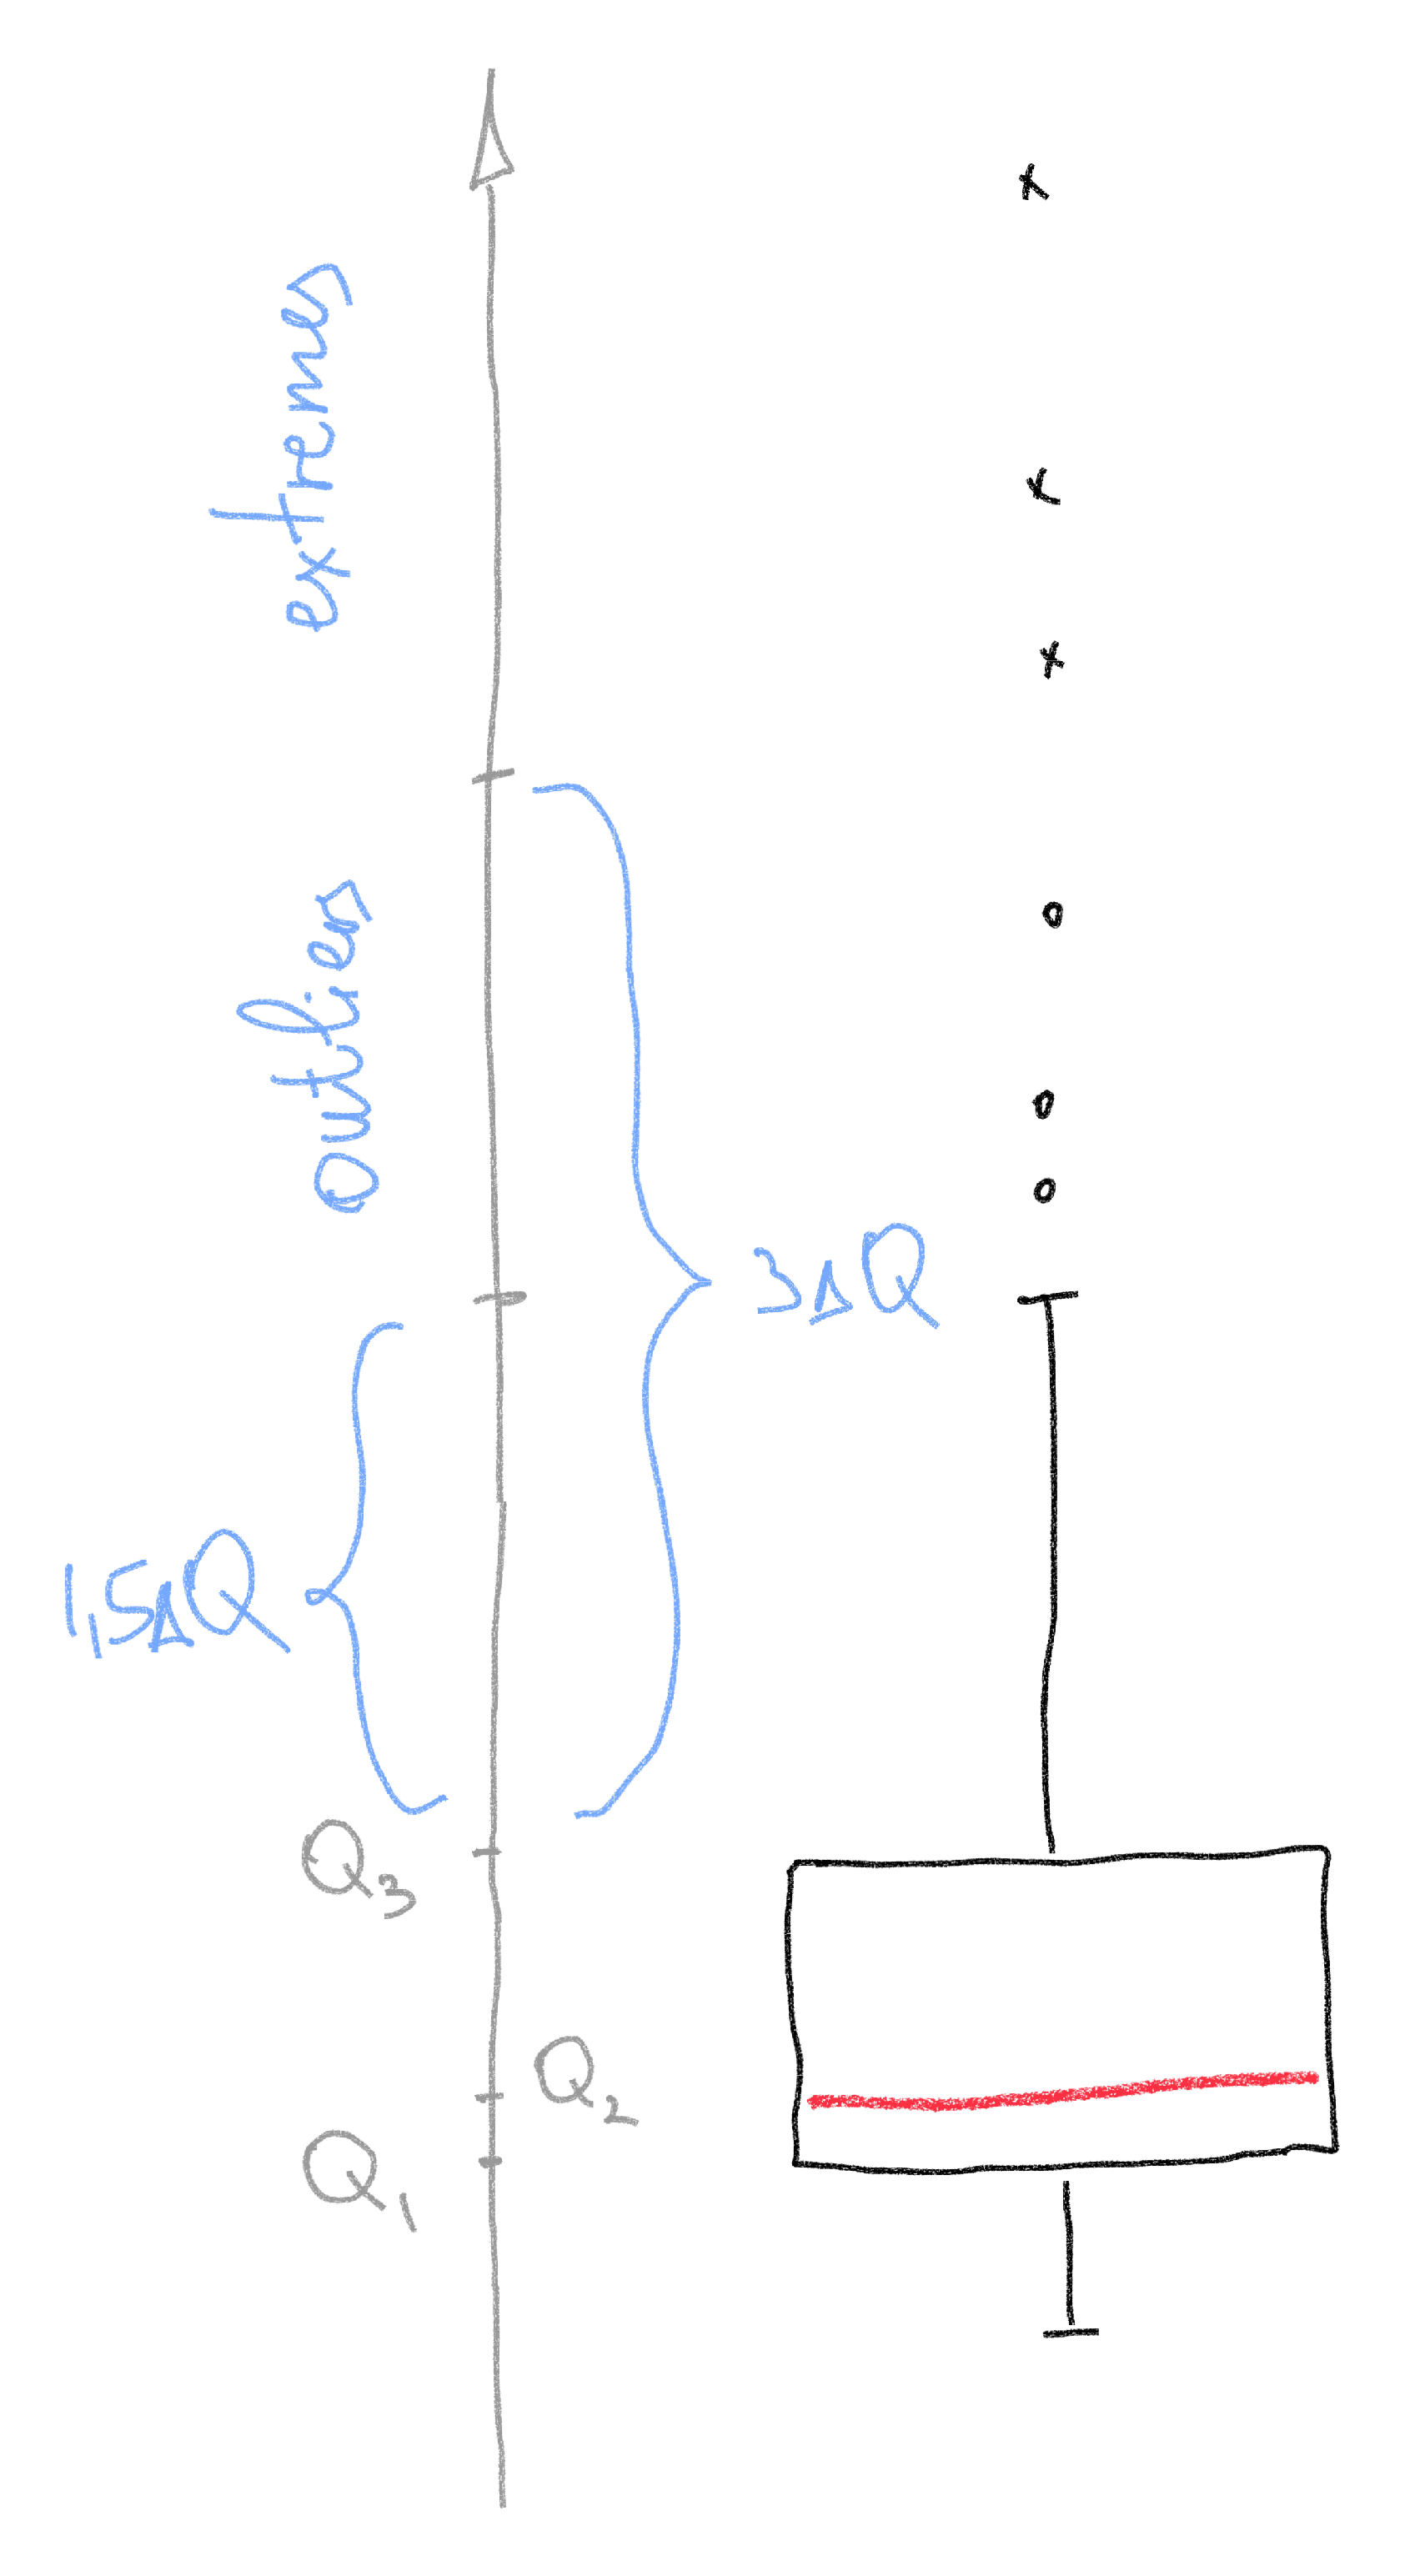
\includegraphics[width=2.7\columnwidth,angle=90]{pics/boxplot.pdf}
    %\caption{Движение $y$}
    \label{fig:boxplot}
\end{marginfigure}

Есть набор наблюдений $x_1, \dots, x_n$, По набору можно вычислить:
\begin{itemize}
    \item $\min$ - минимальное наблюдение
    \item $\max$ - максимальное наблюдение
    \item $M$ - медиана
    \item $Q_1$ - первый квартиль (25\%)
    \item $Q_3$ - третий квартиль (75\%)
\end{itemize}

\emph{Межквартильный размах} задается разностью $\Delta Q = Q_3 - Q_1$.

Длина правого усика, это минимум между расстоянием от квартиля $Q_3$ до
максимального элемента и полутора полуторным межквартильным расстоянием.
Аналогично расчитывается длина правого усика.
\[l = \min(\max(x_i) - Q_3, 1.5 \Delta Q)\]
\[r = \min(Q_1 - \max(x_i), 1.5 \Delta Q)\]
Данные за усиками это \emph{выбросы}, а если они вышли за три межвартильных
расстояния это \emph{чрезвычайные выбросы}.

В ящике с усами используется медиана вместо матожидания\sidenote{Усеченное
    среднее. Если из выборки удалить 2,5\% самых маленьких наблюдений и 2,5\%
    самых больших, то выбросы уже не так сильно будут влиять на вычисленное
матожидание.} в качестве описания потому, что она устойчива к
выбросам.

\section{Кластерный анализ}
\begin{marginfigure}
    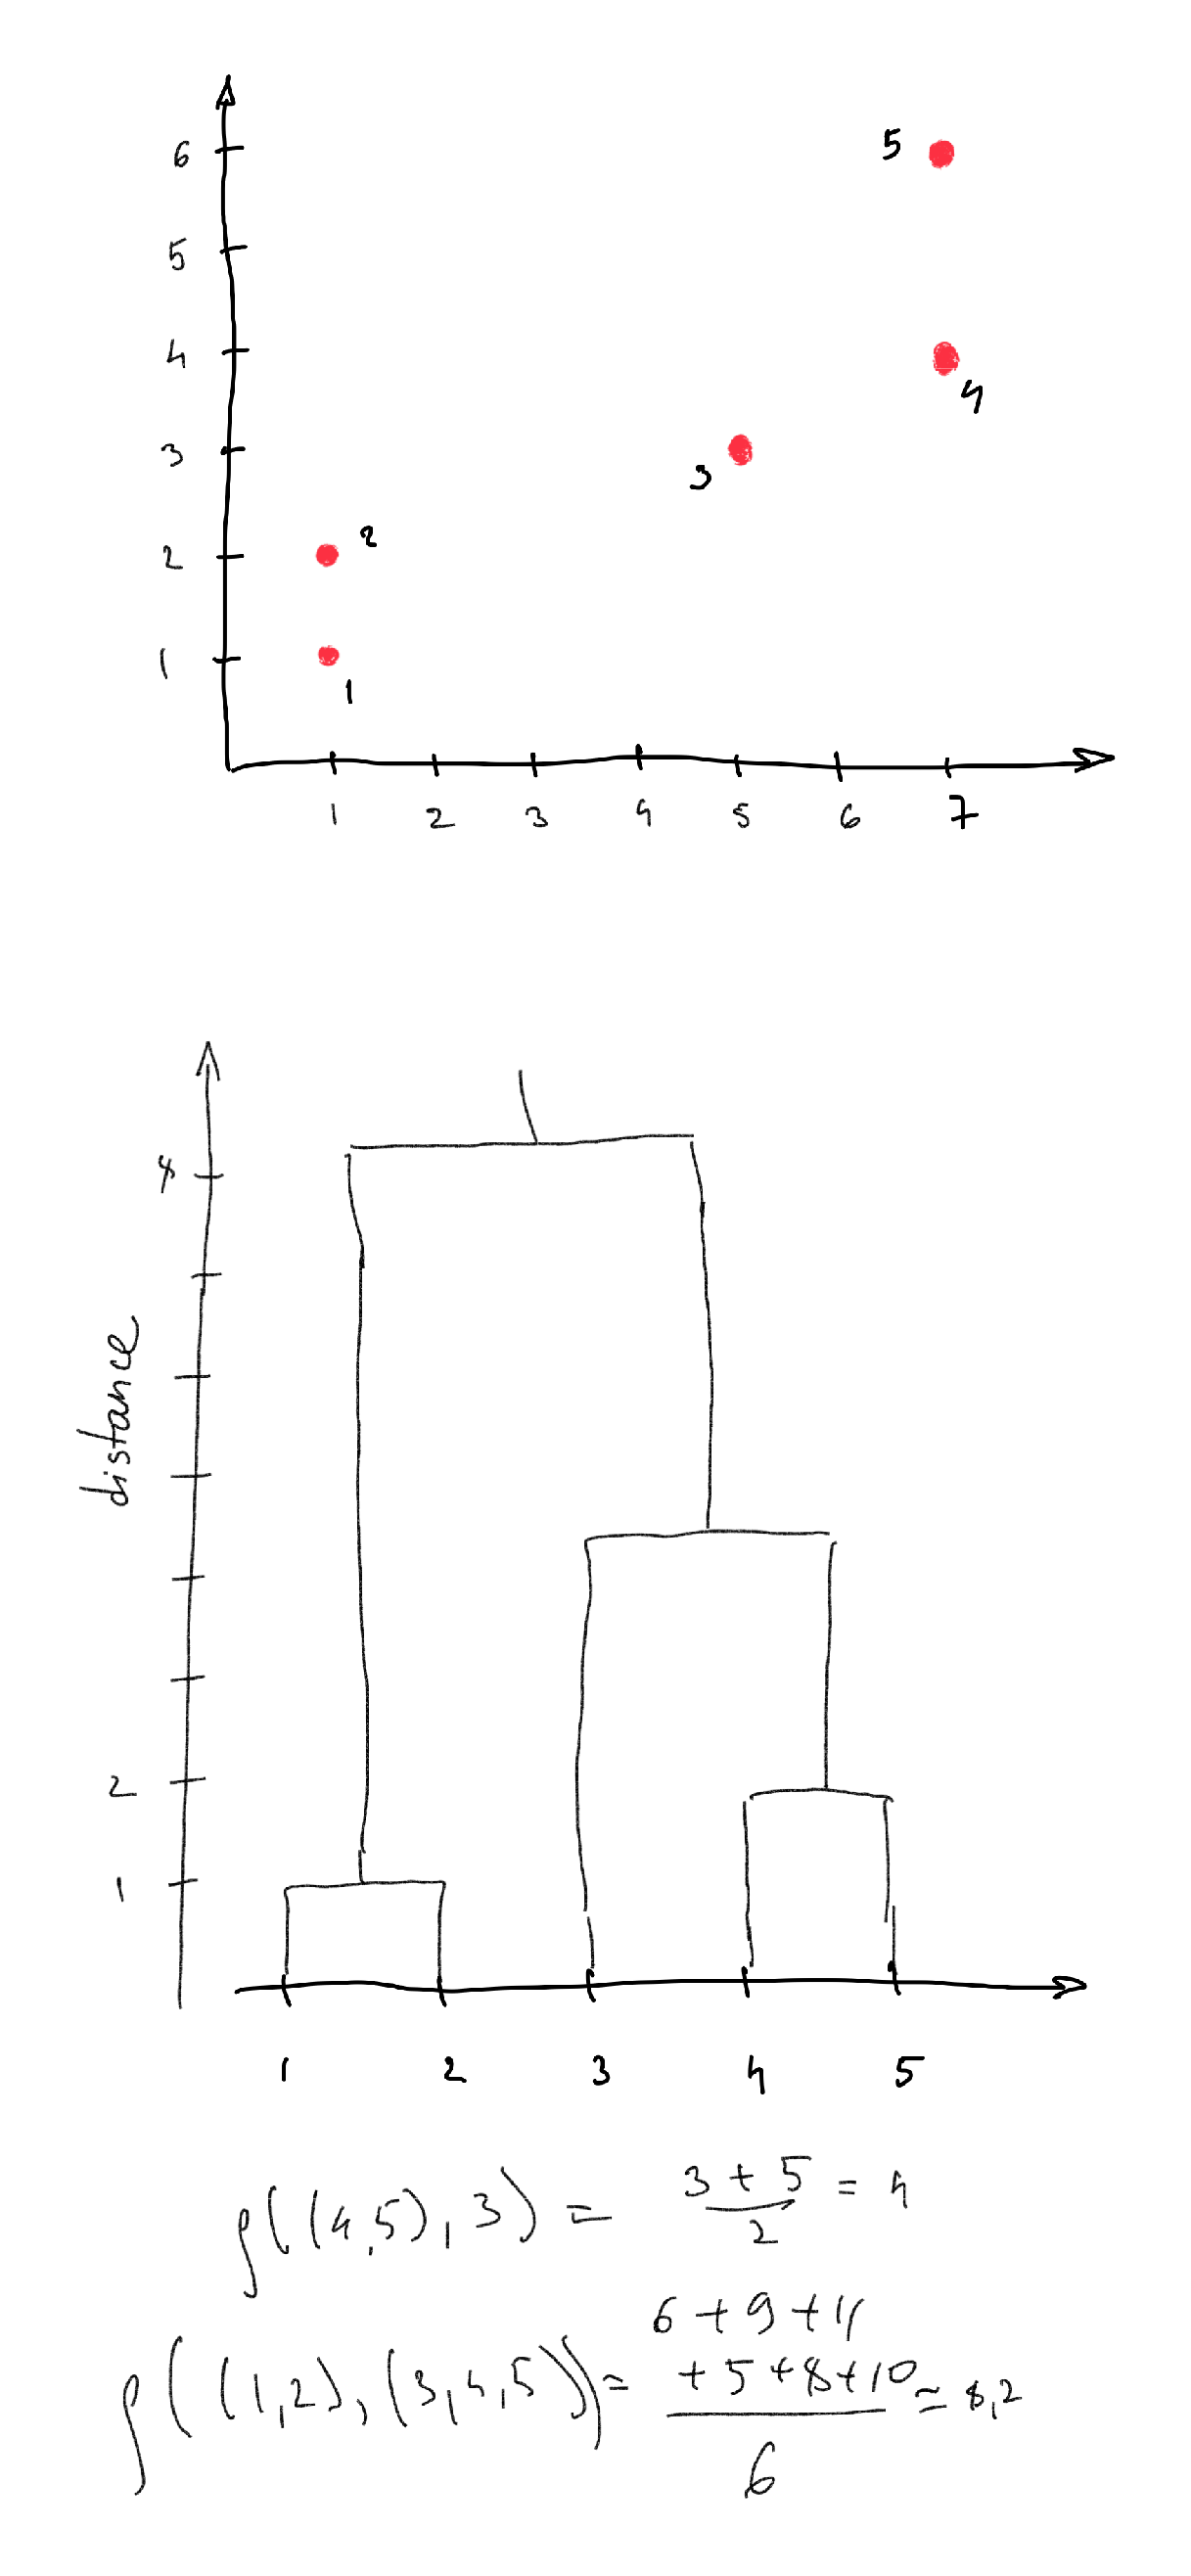
\includegraphics[width=1.1\columnwidth]{pics/dendrogram.pdf}
    %\caption{Движение $y$}
    \label{fig:boxplot}
\end{marginfigure}
Расстояния между кластерами могут быть заданы по разному и стоит обращать
внимание на решаемую задачу. Чтобы задать расстояние между кластерами надо
определить расстояние между точками и на ее основе определить метод построения
кластерного расстояния. Чаще всего используют такие методы:

\begin{itemize}
    \item среднее невзвешенное расстояние (average linkage clustering) -
        среднее расстояние между парами из различных кластеров

    \item центроид метод (устаревший) - расстояние между кластерами
        определяется как расстояние между центрами масс.

    \item метод дальнего соседа (complete linked clustering) - по расстоянию
        между максимально удаленными точками кластеров

    \item метод ближайшего соседа (single linkage clustering) - по расстоянию
        между самыми близкими точками

    \item метод Варда (Ward's method)
\end{itemize}

Дендрограмма выращивается снизу вверх. Сперва каждая точка представляет свой
собственный кластер. Если при достижении уровня $h$ расстояние между точками
равно $h$ то точки объединяются в один кластер (на рисунке это спайка). Процесс
повторяется до тех пор пока не останется один единственный кластер.

Для определения количества кластеров используют метод \emph{плеча}. Для этого
строится график где по оси абсцисс отмечаются шаги объединения (первое
объединение, второе и так далее), по оси ординат откладывается высота на
котором произошло объединение кластеров. На графике ищется точка перелома,
когда расстояние резко увеличивается. Это количество кластеров в данных по
методу локтя.
\sidenote{Результаты кластерного анализа нужно интерпретировать: анализ всегда
должен давать что-то новое о данных, что общего у объектов в кластере и чем
различаются кластеры.}

Недостатки иерархической кластеризации:
\begin{itemize}
    \item Плохо справляется с данными которые вытянуты в длинные ленты в
        простраснтве

    \item Для вычисления требуется хранить попарные расстояния между объектами.
\end{itemize}


\end{document}
